\documentclass{article}
\usepackage[british]{babel}
\usepackage{times}
\usepackage{amsmath}
\usepackage{mathtools}
\usepackage{amsfonts}
\usepackage{verbatim}
\usepackage{lmodern}
\usepackage{tikz}
\usetikzlibrary{patterns}


\DeclareMathOperator*{\argmax}{arg\,max}
\DeclareMathOperator*{\argmin}{arg\,min}

\DeclareMathOperator*{\KL}{{\rm KL}}

\begin{document}
\section{Bayesian inference}
When using Bayesian statistics, one of the often used tools is integrals. However, it usually is a problem as they are not amenable, except in some particular cases, and need to be approximated. Markov Chain Monte Carlo (MCMC) algorithms are the most used and are fairly quick and accurate when working on reasonably small datasets. When the dataset dimensions grow, however, the MCMC algorithms become really time-consuming up to not being computable.\\
\newline
%
When performing MCMC inference, likelihoods and sometimes gradients need to be calculated at each iterations, the cost of these calculations increases with the number of parameters. Moreover, the more dimensions our problem has, the less exact our approximations become, which leads to more iterations to keep the precision needed. For the algorithm to end, all the parameters need to have converged, which means all parameters need to be checked and stored, which is close to impossible when their number is really high.\\
\newline
Another way to perform Bayesian inference is using deterministic methods. It consists in turning the inference problem into an optimization problem. Variational inference belongs to these kind of methods.
% ==========================================================================================
\subsection{Variational inference}
When computing the posterior density of parameters $\boldsymbol{\theta}$ according to observed data $\boldsymbol{y}$, variational inference simplifies the computation by approximating the posterior density $p(\boldsymbol{\theta}\mid \boldsymbol{y})$ with a simpler density $q(\boldsymbol{\theta})$. One way to do so is the variational inference, which gives an approximation of the posterior distribution as a result of an optimization problem that minimizes a measure of "closeness" as objective function.\\
\newline
%
We suppose we have observations $y$ and parameters $\boldsymbol{\theta}$, we are looking to determine the posterior distribution of the parameters conditional on the observations $p(\boldsymbol{\theta} \mid \boldsymbol{y})$. Given a family of densities $\mathcal{D}$ over the parameters, we want to find the distribution $q \in \mathcal{D}$ that minimizes the "closeness" measure compared to $p(\boldsymbol{\theta} \mid \boldsymbol{y})$.\\
\newline
%
Variational inference minimizes the Kullback-Leibler divergence as a "closeness" measure. Introduced in 1951 by Kullback and Leibler\cite{kl51}, it is the most common divergence measure used in statistics and machine learning. It is described as such:
\begin{equation*}
\KL(p\parallel q) := \int q(\boldsymbol{\theta})\log \left(\frac{q(\boldsymbol{\theta})}{p(\boldsymbol{\theta} \mid \boldsymbol{y})}\right) \mathrm{d}\boldsymbol{\theta}.
\end{equation*} 
It is described as a "directed divergence" as it is asymmetric, \textit{i.e.} $\KL(p\parallel q) \neq \KL(q \parallel p)$.\\
\newline
%
Determining the family $\mathcal{D}$ can be tricky as we need the family to be simple enough to be optimized efficiently, but flexible enough for the approximation $q \in \mathcal{D}$ to be close to $p(\boldsymbol{\theta} \mid \boldsymbol{y})$ w.r.t the KL divergence.\\
\newline
%
The approximation will then be:
\begin{equation*}
q^*(\boldsymbol{\theta} ) = \argmin_{q(\boldsymbol{\theta}) \in \mathcal{D}} \KL\left( q(\boldsymbol{\theta}) \parallel p(\boldsymbol{\theta} \mid \boldsymbol{y})\right).
\end{equation*}
Minimizing the KL divergence can be complicated depending on the density $p$ we want to approximate and the densities family $\mathcal{D}$ we want $q$ to be apart of. We can decompose the KL divergence as follows:
\begin{align*}
\KL\left(q(\boldsymbol{\theta})||p(\boldsymbol{\theta}\mid \boldsymbol{y})\right) &= \mathbb{E}\left[\log q(\boldsymbol{\theta})\right] - \mathbb{E}\left[\log p(\boldsymbol{\theta}\mid \boldsymbol{y})\right],\\
&= \mathbb{E}\left[\log q(\boldsymbol{\theta})\right] - \mathbb{E}\left[\log p(\boldsymbol{y},\boldsymbol{\theta})\right] + \log p(\boldsymbol{y}).
\end{align*}
We introduce the evidence lower bound (\small{ELBO}):
\begin{align*}
\mathcal{L}(q) &= \mathbb{E}\left[\log p(\boldsymbol{\theta},\boldsymbol{y})\right] - \mathbb{E}\left[\log q(\boldsymbol{\theta})\right],\\
&=\int q(\boldsymbol{\theta})\log\frac{p(\boldsymbol{y},\boldsymbol{\theta})}{q(\boldsymbol{\theta})}\mathrm{d}\boldsymbol{\theta}.
\end{align*}
When decomposing the KL divergence, we obtain:
\begin{equation*}
\KL(q\parallel p) = \log(p) - \mathcal{L}(q).
\end{equation*}
This means that the KL divergence is the difference between the marginal log-likelihood with no effect on the optimization and a function : $\mathcal{L}(q)$. So minimizing the KL divergence is the same as maximizing $\mathcal{L}(q)$. The difference lays in the complexity of the problems, minimizing the KL divergence is not tractable, but maximizing $\mathcal{L}(q)$ admits a closed form when the family of densities $\mathcal{D}$ is well chosen. In such a case, we prefer to use $\mathcal{L}(q)$ as an objective function.\\
\newline
%
Using Jensen's inequality, we can show that $\mathcal{L}(q)$ is a lower bound for the marginal log-likelihood, which is why we call it the evidence lower bound, or variational lower bound.
\begin{align*}
\log p(\boldsymbol{y}) &= \log \int p(\boldsymbol{y}, \boldsymbol{\theta}) \mathrm{d}\boldsymbol{\theta},\\
&= \log \int \frac{p(\boldsymbol{y}, \boldsymbol{\theta})}{q(\boldsymbol{\theta})}q(\boldsymbol{\theta})\mathrm{d}\boldsymbol{\theta}
,\\
&\geq \int q(\boldsymbol{\theta}) \log \left\lbrace \frac{p(\boldsymbol{y}, \boldsymbol{\theta})}{q(\boldsymbol{\theta})} \right\rbrace \mathrm{d}\boldsymbol{\theta},\\
&= \mathcal{L}(q).
\end{align*}
Hence, $\log p(\boldsymbol{y}) \geq \mathcal{L}(q)$, justifying the name "lower bound" for $\mathcal{L}(q)$.
%
\subsection{Mean-field approximation}
The complexity of the optimization problem is directly bound to the complexity of the family of densities $\mathcal{D}$ we want $q(\boldsymbol{\theta})$ to be apart of. We introduce the mean-field variational family, where the parameters are mutually independent and are governed by a distinct factor in the variational density.\\
\newline
Let's call $\left\lbrace \theta_j\right\rbrace_{j=1}^J$ a partition of $\boldsymbol{\theta}$, if $q \in \mathcal{D}$ and $\mathcal{D}$ a mean-field variational family, then:
\begin{equation*}
q(\boldsymbol{\theta}) = \prod_{j=1}^J q_j(\theta_j)
\end{equation*}
We determine the variational factors $q_j(z_j)$ by maximizing $\mathcal{L}(q_j)$. Hence, the variational family does not directly represent the observed data, they are both linked through the optimization of the \small{ELBO}.\\
\newline
%
To visualise the mean-field approximation, we consider a two dimensional Gaussian distribution, represented in clear in Figure \ref{fig:mean_field}. The mean-field approximation of the posterior distribution is represented by the barred circle. We can see that the mean of the approximation is the same as the real mean, but the covariance doesn't match the covariance of the real posterior.\\
\newline
%
\begin{figure}[h!]
\centering
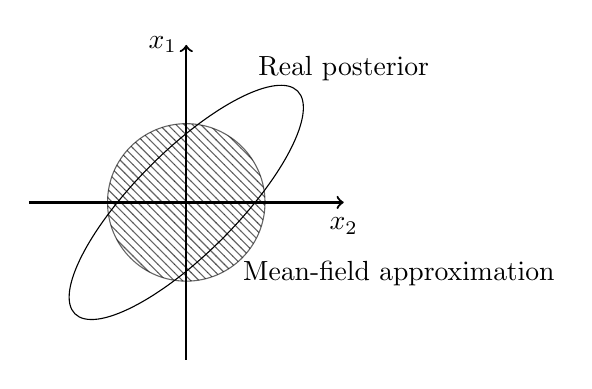
\begin{tikzpicture}
\draw[thick, ->] (0,-2) -- (0,2);
\draw[thick, ->] (-2,0) -- (2,0);
\fill[pattern=north west lines,opacity=.6,draw] (0,0) circle (1cm);
\draw[rotate=-45] (0,0) ellipse (0.65cm and 2cm);
\node (p) at (2,1.7) {Real posterior};
\node (q) at (2.7,-0.9) {Mean-field approximation};
\node (x1) at (-0.3,2) {$x_1$};
\node (x2) at (2,-0.3) {$x_2$};
\end{tikzpicture}
\caption{\label{fig:mean_field}Visualisation of mean-field approximation to a two-dimensional Gaussian posterior. The correlations in the mean-field approximation do not represent the correlations of the real posterior.}
\end{figure}
%
We have transformed, using the \small{ELBO} and the mean-field approximation our problem into a optimization problem. We now need a way to solve this problem. In the following section, we will be looking at the coordinate ascend mean-field variational inference.
% =========================================
\subsection{Coordinate ascent mean-field variational inference \small{(CAVI)}}
The coordinate ascent mean-field variational inference (\small{CAVI}) is one of the most common used to solve this kind of optimization problem. The algorithm iterates on the parameters of the mean-field approximation, optimizing them one at the time. It yields a local optimum for the \small{ELBO}.\\
\newline
The \small{ELBO} is based on the following result:
% =========================================
\newpage
\section{Results}
\begin{figure}
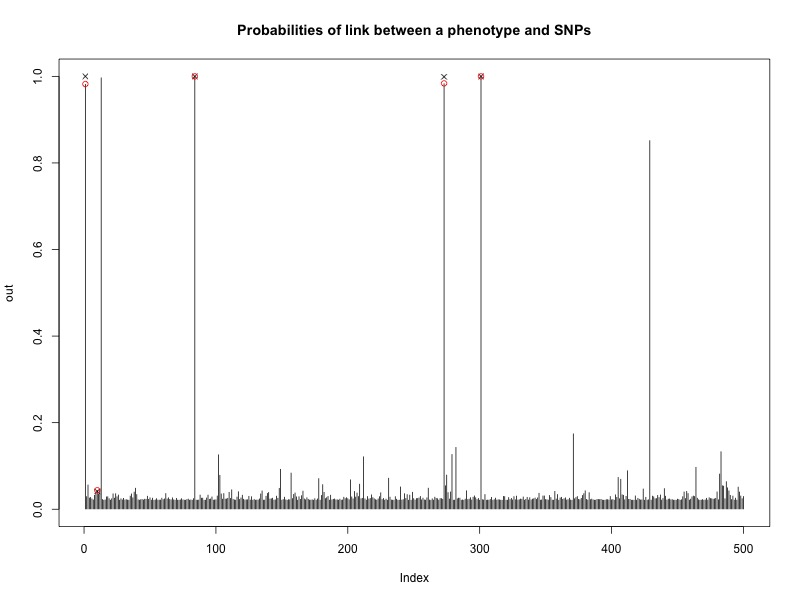
\includegraphics[width=5in]{images/multipleProba1.jpg}
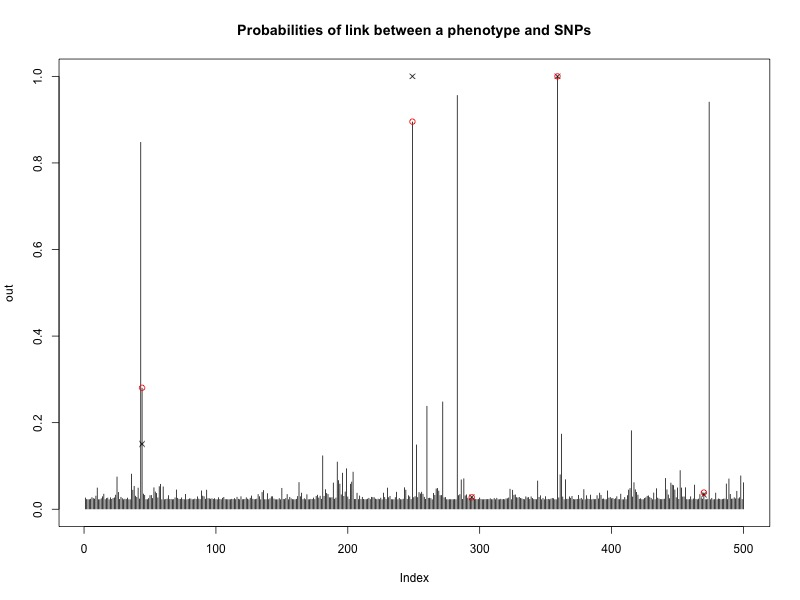
\includegraphics[width=5in]{images/multipleProba2.jpg}
\end{figure}

\begin{figure}
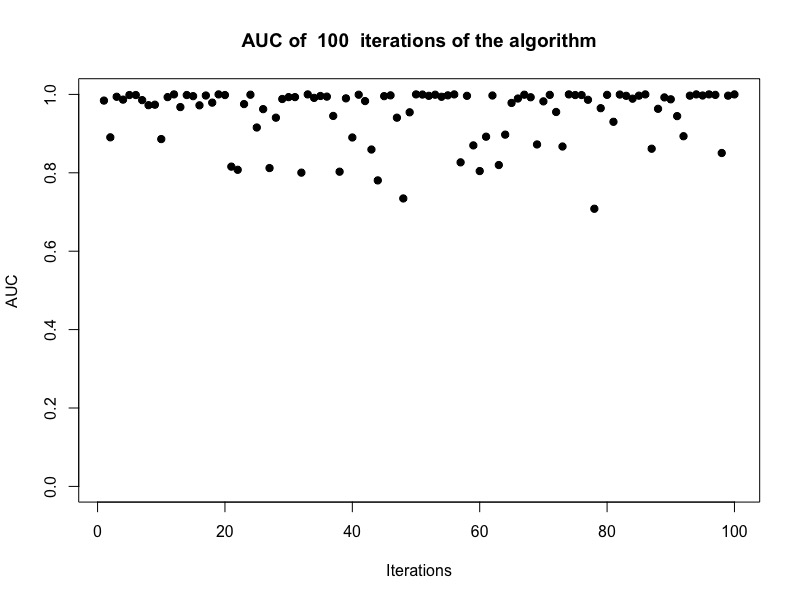
\includegraphics[width=5in]{images/AUC_100_iter.jpeg}
\end{figure}

\begin{figure}
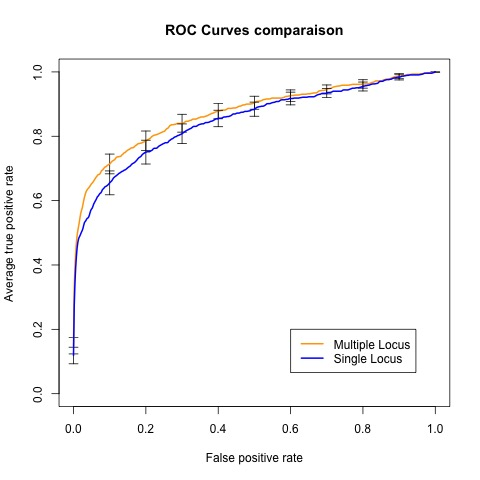
\includegraphics[width=2.7in]{images/ROC_Comp_p0_15_var_0_5.jpeg}
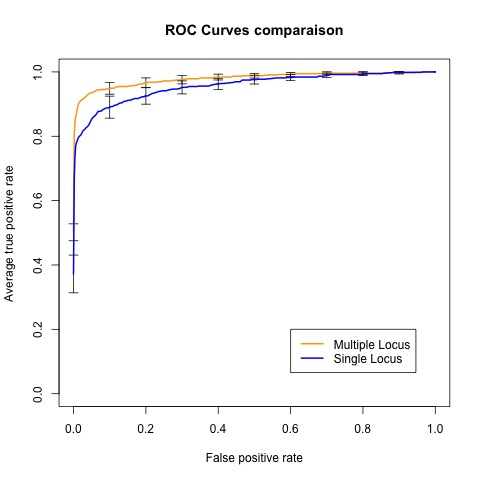
\includegraphics[width=2.7in]{images/ROC_Comp_p0_15_var_0_8.jpeg}
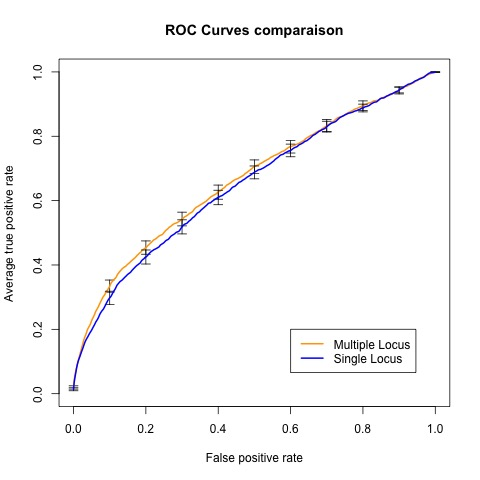
\includegraphics[width=2.7in]{images/ROC_Comp_p0_50_var_0_5.jpeg}
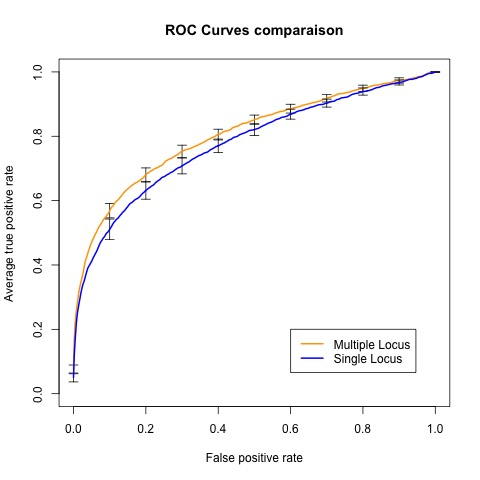
\includegraphics[width=2.7in]{images/ROC_Comp_p0_50_var_0_8.jpeg}
\caption{Top: $p_0 = 15$, Left: Max tot. PVE$ = 0.5$,
Bottom: $p_0 = 50$, Right: Max tot. PVE$ = 0.8$}
\end{figure}
% =========================================
\newpage
%\bibliography{references}
%\bibliographystyle{plain}
\end{document}